\documentclass{article}
\usepackage{tikz}
\usetikzlibrary{arrows.meta, positioning}

\begin{document}

\begin{figure}[h]
    \centering
    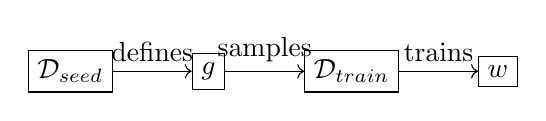
\begin{tikzpicture}[node distance=1cm, auto]
        % Define nodes
        \node[draw, align=center] (D_seed) {$\mathcal{D}_{\text{seed}}$};
        \node[draw, right=of D_seed] (G) {$g$};
        \node[draw, right=of G] (D_train) {$\mathcal{D}_{\text{train}}$};
        \node[draw, right=of D_train] (W) {$w$};

        % Draw edges
        \path[->] (D_seed) edge node {defines} (G);
        \path[->] (G) edge node {samples} (D_train);
        \path[->] (D_train) edge node {trains} (W);
    \end{tikzpicture}
    \hspace{2cm}
    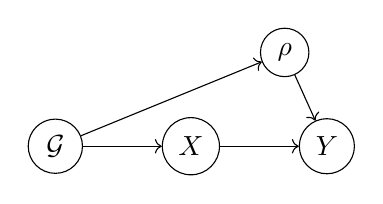
\begin{tikzpicture}[node distance=1cm, auto]
        % Define nodes
        \node[draw, circle] (G) {$\mathcal{G}$};
        \node[draw, circle, right=of G] (X) {$X$};
        \node[draw, circle, above right=of X] (rho) {$\rho$};
        \node[draw, circle, right=of X] (Y) {$Y$};

        % Draw edges
        \path[->] (G) edge node {} (X);
        \path[->] (G) edge node {} (rho);
        \path[->] (rho) edge node {} (Y);
        \path[->] (X) edge node {} (Y);
    \end{tikzpicture}
    
    \caption{Left: Data generation pipeline. Right: The fine-tuned network $q_\theta$ learns to do inference in a graphical model where the prior over programs, $\mathcal{G}$, is defined by prompting an LLM with example code in $\mathcal{D}_\text{seed}$, while the likelihood $p(Y|\rho, X)$ is defined by program execution.}
\end{figure}

\end{document}